\documentclass[11pt,dvipdfmx]{jreport}
\usepackage{wuse_thesis}
\usepackage{indentfirst}
\usepackage{url}	% \url{}コマンド用.URLを表示する際に便利
\usepackage{graphicx}  % ←graphicx.styを用いてEPSを取り込む場合有効にする
\usepackage{listings,jvlisting} %日本語のコメントアウトをする場合jvlisting(もしくはjlisting)が必要

\usepackage{multirow}

\usepackage{color}

\renewcommand{\lstlistingname}{Program}
\newcommand{\todo}[1]{\colorbox{yellow}{{\bf TODO}:}{\color{red} {\textbf{[#1]}}}}
			% 他のパッケージ・スタイルを使う場合には適宜追加

%ここからソースコードの表示に関する設定
\definecolor{darkgray}{rgb}{.4,.4,.4}
\definecolor{purple}{rgb}{0.65, 0.12, 0.82}

\lstdefinelanguage{JavaScript}{
  keywords={typeof, new, true, false, catch, function, return, null, catch, switch, var, if, in, while, do, else, case, break},
  keywordstyle=\color{blue}\bfseries,
  ndkeywords={class, export, boolean, throw, implements, import, this},
  ndkeywordstyle=\color{darkgray}\bfseries,
  identifierstyle=\color{black},
  sensitive=false,
  comment=[l]{//},
  morecomment=[s]{/*}{*/},
  commentstyle=\color{purple}\ttfamily,
  stringstyle={\small\ttfamily},
  morestring=[b]',
  morestring=[b]"
}

\lstset{
  basicstyle={\ttfamily},
  identifierstyle={\small},
  commentstyle={\smallitshape},
  keywordstyle={\small\bfseries},
  ndkeywordstyle={\small},
  stringstyle={\small\ttfamily},
  frame={tb},
  breaklines=true,
  columns=[l]{fullflexible},
  numbers=left,
  xrightmargin=0zw,
  xleftmargin=3zw,
  numberstyle={\scriptsize},
  stepnumber=1,
  numbersep=1zw,
  lineskip=-0.5ex
}
%ここまでソースコードの表示に関する設定

%%%%%%%%%%%%%%%%%%%%%%%%%%%%%%%%%%%%%%%%%%%%%%%%%%%%%%%%%%%%%%%%%%%%%%%%

%%%%%%%%%%%%%%%%%%%%%%%%%%%%%%%%%%%%%%%%%%%%%%%%%%%%%%%%%%%%%%%%%%%%%%%%

%%
%% 主に表紙を作成するための情報
%%

%%  タイトル(修論の場合は英語表記も指定)
\title{JavaScriptテストコード変更内容に基づく\\後方互換性損失の検出}
%\etitle{Test\\Test\\Test}

%%  著者名(修論の場合は英語表記も指定)
\author{前川 大樹}
%\eauthor{Akinori Ihara}

%% 卒業論文・修士論文(以下のどちらかを選択)
\bachelar	% 卒業論文(4年生用)
%\master  	% 修士論文(M2用)

%%  学科・クラスタ
\department{システム工}
%\department{デザイン情報}
%\department{デザイン科学}

%%  学生番号
\studentid{60256245}

%%  卒業年度
\gyear{2023}		% 提出年が2022年なら,2021年度

%%  論文提出日
\date{2024年2月13日}	% 修士の場合は月(2021年2月)までとし,英語表記も指定
%\edate{February 2021}	% 修士の場合,こちら(英語表記)も有効化

%%%%%%%%%%%%%%%%%%%%%%%%%%%%%%%%%%%%%%%%%%%%%%%%%%%%%%%%%%%%%%%%%%%%%%%%

\begin{document}

\maketitle

%%
%%  概要
%%
\begin{abstract}
  本研究では,ソフトウェアの後方互換性の損失をテストコードの変更内容に基づいて判定する手法を提案する.

  ソフトウェア開発では,ライブラリと呼ばれる再利用可能なプログラムの利用により,開発者自身が同じ機能を再実装する必要がなくなり開発効率が向上する.ライブラリに対して行われる変更は,軽微な修正であっても破壊的変更が含まれることがあり,変更後のライブラリが後方互換性を維持しているか否かをライブラリ利用者が正確に判断することは困難である.

  従来研究では,ライブラリの動作を検証するテストコードの変更有無に着目した後方互換性の損失の判定手法を提案している.しかし,テストコードはテストの誤り修正や実行手順の変更など,ライブラリの変更とは無関係に変更されることがあり,従来手法ではテストコードの変更内容は考慮されておらず誤検出が多い.

  本研究では,従来研究の誤検出を減らすために,テストコードの変更内容を考慮した後方互換性の判定手法を提案する.具体的には,後方互換性が損失するライブラリバージョンにおけるテストコードの変更内容を明らかにし,自動検出するツールを開発して後方互換性の損失の判定精度を検証する.

\end{abstract}

%%  目次
\tableofcontents

%%  図目次 (図目次をいれたければ以下のコメントをはずす)
%\listoffigures

%%  表目次 (表目次をいれたければ以下のコメントをはずす)
%\listoftables

\newpage
\pagenumbering{arabic}	% 以降のページ番号を算用数字に

%%%%%%%%%%%%%%%%%%%%%%%%%%%%%%%%%%%%%%%%%%%%%%%%%%%%%%%%%%%%%%%%%%%%%%%%

%%
%%  本文はここから
%%

\chapter{はじめに}
ソフトウェア開発では,ライブラリと呼ばれる再利用可能なプログラムの利用により,開発者自身が同じ機能を再実装する必要がなくなり開発効率が向上する.ライブラリは機能追加やバグ修正により頻繁に更新されており,利用者は適宜ライブラリのバージョン更新が必要である.利用者が安全にライブラリを更新するために,パッケージマネージャはセマンティックバージョニング\footnote{\url{https://semver.org}}を採用し,バージョン間の互換性の有無を管理している.セマンティックバージョニングでは,ライブラリ更新をメジャー,マイナー,パッチのレベルに分類し,マイナーとパッチの更新では後方互換性を保つ変更が求められる.しかし,バージョン名の付与は開発者が手動で行うため,後方互換性が損失しているにも関わらず,誤ってマイナーやパッチに分類されてしまうことがある.
この問題は,特にJavaScriptのような動的な言語において顕著であり,ライブラリと利用者のコードの不整合が実行時まで検出されないという課題がある.
この課題に対して,JavaScriptライブラリの後方互換性を判定する研究が行われている.

松田らは,後方互換性を損失するライブラリの更新は,プログラムの更新と合わせてテストコードも修正すると考え,テストコードの変更有無による後方互換性の判定手法を提案した.
\cite{matsuda}
しかし,テストコードの変更内容を考慮しておらず,テストの誤り修正や実行手順の修正など,ライブラリ変更とは無関係のテストコード変更についても後方互換性を損失したと誤検出する.

本研究では,テストコードの変更内容に着目し,後方互換性の損失に関係するテスト変更内容を明らかにし,テスト変更内容に基づく後方互換性の判定手法の精度を評価する.具体的には,2つのリサーチクエスチョン(RQ)に回答する.

\begin{itemize}
  \item RQ1:後方互換性の損失に関係するテストコード変更とは何か?
  \item RQ2:テストコード変更内容に基づく後方互換性の判定手法の有効性はどの程度か?
\end{itemize}

\chapter{後方互換性の損失}

\section{クライアントへの影響}
ライブラリの後方互換性の損失とは,ライブラリのバージョン更新によって,更新前のバージョンとの互換性が損なわれることを指す.クライアントソフトウェアは,更新前のライブラリ仕様を前提とするため,後方互換性を損失するライブラリのバージョン更新を適用する際,コードの不整合によるエラーが起きることがある.この問題に対して,ライブラリ開発者は後方互換性の損失を含むライブラリ更新をクライアントに正確に伝えることが求められる.

ライブラリ開発者がクライアントに後方互換性の損失を伝える手法として,セマンティックバージョニング\footnote{\url{https://semver.org}}がある.セマンティックバージョニングは,バージョン名を付与するための規則でバージョン名はそのソフトウェアの変更点や互換性に関する情報を提供する.バージョン名は,{\verb|MAJOR.MINOR.PATCH|}の形式をとる.後方互換性を損失する変更では{\verb|MAJOR|},後方互換性を保つ変更では{\verb|MINOR|}または{\verb|PATCH|}の値を増やすことで後方互換性の有無をクライアントに伝える.

ライブラリ更新をメジャー,マイナー,パッチのレベルに分類し,バージョン名によって後方互換性の有無を,後方互換性を損失する変更ではメジャーを,後方互換性を保つ変更ではマイナーバージョンもしくはパッチバージョンを更新する.しかし,バージョン名の付与はライブラリ開発者が手動で行うため,後方互換性が損失しているにも関わらず誤ってマイナーやパッチに分類されてしまうことがある.



\section{後方互換性の損失の原因}
クライアントソフトウェアの開発者が依存ライブラリのバージョン更新を取り込む際,クライアントは更新前のライブラリ仕様を前提とするため不整合によるエラーが起きることがある.この問題に対して,ライブラリ開発者は利用者に影響があるライブラリ変更を意図せずバージョン更新に含めないことが求められる.

ライブラリ開発者によって新しいライブラリバージョンがリリースされた際,更新前のライブラリ仕様を前提としたクライアントソフトウェアとの不整合が起きることがある.

更新前のライブラリ仕様を前提としたクライアントと,更新後の


ライブラリの後方互換性の損失とは,新しいバージョンのライブラリがリリースされた際に,以前のバージョンとの互換性が損なわれることを指す.後方互換性を損失する更新が入ったライブラリバージョンをクライアントソフトウェアが適用すると,クライアントソフトウェアが期待通りに動作しなくなることがあるため,ライブラリ開発者は意図せず後方互換性を損失する変更をバージョン更新に含めないことが求められる.

\section{関連研究}

\subsection{ライブラリ変更に基づく後方互換性の検出手法}

\subsection{テストケースに基づく後方互換性の検出手法}

\section{キーアイデア}

\chapter{RQ1:後方互換性の損失を伴わないテストコード変更とは何か?}\label{rq1}

\section{概要}
本章では,従来研究で誤検出となる,後方互換性の損失を伴わないテストコード変更が存在するか分析する.具体的には,各ライブラリバージョンに対して,後方互換性の有無の判定と,テストコード変更内容を集計する.各バージョンのテストコードの変更内容は,テストコードの変更差分から目視により分類する.後方互換性の有無の判定はMujahidらの提案手法を使用する.

\section{分析手法}
本分析では,各ライブラリ更新ごとに後方互換性の判定と,テストコード変更内容を目視により集計する.

\subsection{テストコード変更内容の目視分類}
テストコード変更内容を目視分類するために,テストコードの構成要素をまとめる.本研究では,プログラムのテストの中でも単体テストを対象とする.単体テストとは,関数やクラスなどのプログラムを構成する単位(ユニット)が開発者の期待通りに動作するかを検証するテスト手法である.単体テストを実施する際は,テスト対象ユニットに対応するテストスイートを用意する必要がある.テストスイートとは,テストの目的や条件が似ているテストケースの集合を指す.テストケースは,テスト項目の最小単位であり,テスト対象への入力と期待される結果(期待値)の組み合わせで構成する.入力値と期待値を受け取ってプログラムが正しく動作しているか検証する仕組みをアサーションと呼ぶ.

\begin{lstlisting}[caption=Calculator.js, label=Calculator.js]
class Calculator {
  add(a, b) {
    return a + b;
  }
}
\end{lstlisting}

\begin{lstlisting}[caption=Calculator.test.js, label=Calculator.test.js]
import { Calculator } from './Calculator';

describe('Calculator', () => {
  let calculator;

  beforeEach(() => {
    calculator = new Calculator();
  });

  test('should add two positive numbers', () => {
    if (calculator) {
      expect(calculator.add(1, 1)).toBe(2);
    }
  });
});
\end{lstlisting}


Program~\ref{Calculator.js},Program~\ref{Calculator.test.js}は,JavaScriptにおけるテストコードの例を示す.Program~\ref{Calculator.js}は,テスト対象となるクラス{\verb|Calculator|}が定義されている.このクラスに含まれるメソッド{\verb|add()|}は,2つの引数を受け取り足し合わせた値を返す関数である.Program~\ref{Calculator.test.js}は,{\verb|Calculator|}クラスを単体テストによって検証するファイルで,JavaScript向けテストフレームワークJest\footnote{\url{https://jestjs.io/}}を使用して記述している.

Program~\ref{Calculator.test.js}に含まれる{\verb|describe|}関数でテストスイートを宣言し,{\verb|test|}関数により1つのテストケースを定義している.テストスイートやテストケースは,何を検証するかが記述されるラベルと,検証するテスト用関数を引数に取る.6行目から7行目の{\verb|beforeEach|}関数で,テストフィクスチャと呼ばれる,テストデータの初期化などのテストの事前条件を定義できる.例では,{\verb|Calculator|}クラスをインスタンス化している.テストケース(10行目から12行目)では,11行目で{\verb|if|}文によりテストの前提条件を記述し,12行目のアサーションで{\verb|Calculator.add()|}に対し{\verb|1|}と{\verb|1|}を入力したときの動作を検証している.この場合,期待する結果は{\verb|2|}であるため,{\verb|toBe|}節で結果が{\verb|2|}となる.

以上を踏まえ,本論文では,テストコードの変更内容として10件の内容を考慮する.

\begin{itemize}
  \setlength{\itemsep}{0cm}
  \item テストスイートの追加
  \item テストスイートの削除
  \item テストケースの追加
  \item テストケースの削除
  \item アサーションの追加
  \item アサーションの削除
  \item アサーションの入力値の変更
  \item アサーションの期待値の変更
  \item テストの前提条件の変更
  \item テストフィクスチャの変更
  \item リファクタリング
\end{itemize}

リファクタリングは,テストスイート・テストケースのラベルの変更,テストフレームワークの変更,可読性向上のためのフォーマッティングなどテストコードの振る舞いに関わらない変更を含む.

\subsection{後方互換性の判定}\label{kouhougokanseinohantei}
後方互換性の判定には,Mujahidらの手法を使用する.Mujahidらは,ライブラリの後方互換性の損失をクライアントテストを実行することで検出する手法を提案した\cite{mujahid}.後方互換性を損失する変更を加えられたライブラリバージョンでは,その影響を受けるクライアントテストの結果が更新前後で成功から失敗に変化することを手法の根拠としている.本分析でも,対象ライブラリのクライアントのデータを収集し,更新前後でクライアントテストを実行する.

\section{データセット}\label{rq1:datasets}
データセットとして,従来研究\cite{matsuda}で収集されたライブラリバージョン群を使用する.従来研究では,ライブラリの人気度を示すnpmスコア~\footnote{\url{https://npms.io}}が上位500件以内で,各バージョンのコミットにおけるテスト実行時の成功率が100%であることを条件にnpm\footnote{\url{https://www.npmjs.com/}}から2,111件のライブラリバージョンを収集した.本調査では,このデータセットから,ライブラリテストに変更があるライブラリバージョン1,027件を抽出し,95%の信頼区間でサンプリングした280件を対象とする.分析対象とするライブラリのいずれかのバージョンに依存するクライアントは,Mujahidらのデータセットから抽出した.

\section{分析結果}
\begin{figure}[t]
  \label{fig:test_pattern}
  \centering
  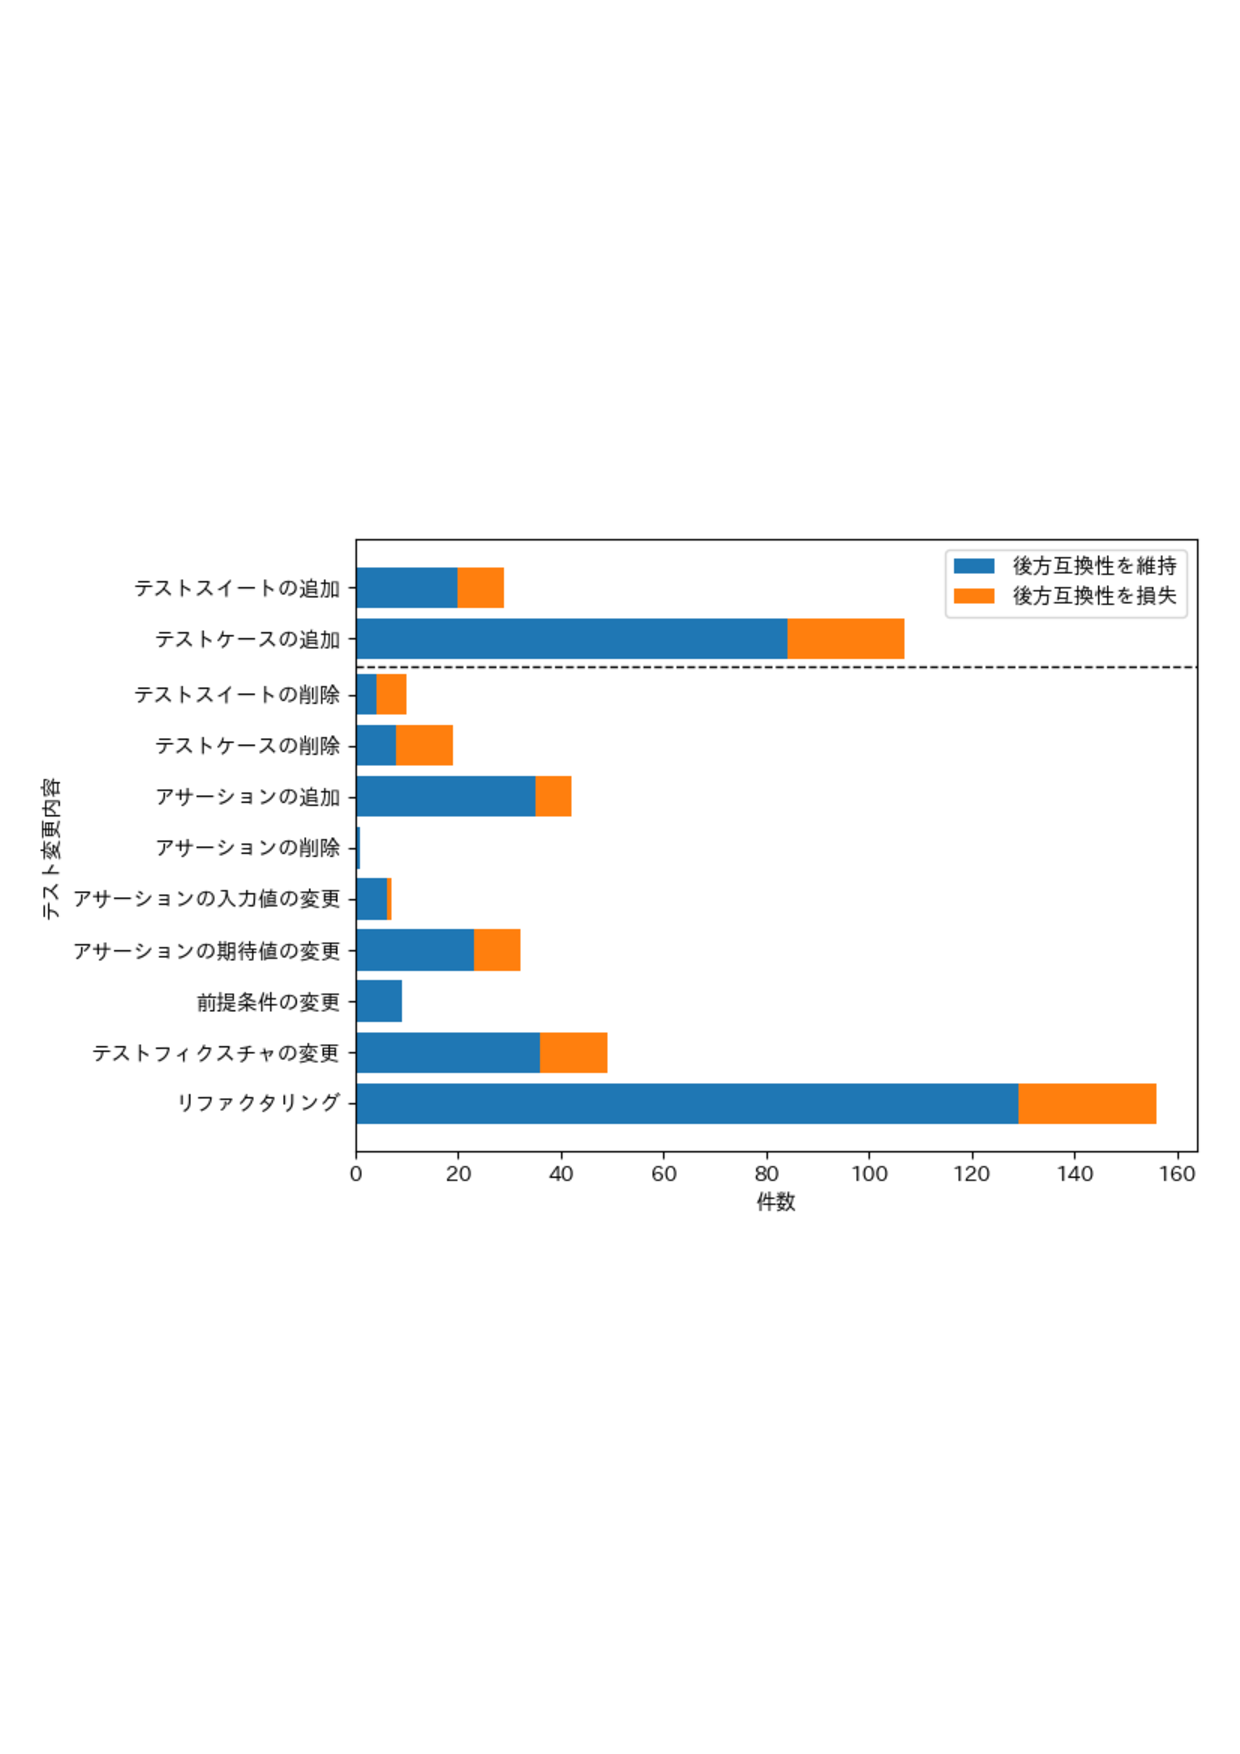
\includegraphics[width=1.0\linewidth]{fig/barh-test-pattern.pdf}
  \caption{テスト変更内容ごとの実際の後方互換性}
\end{figure}

\todo{以下TODO}
図\ref{fig:test_pattern}は,テスト変更内容ごとの後方互換性の有無を横棒積み上げ棒グラフで示す.縦軸は各変更内容,横軸は発生件数である.リファクタリングは件数も多くほとんどが実際に後方互換性を保っているため,後方互換性の損失に関係するテスト変更とは言えず,従来研究の手法で誤検出となる大きな原因であるとわかる.テストスイートの削除,テストケースの削除は,後方互換性なしの割合が後方互換性ありの割合より高く,後方互換性の損失と関係のあるテストコード変更と言える.また,アサーションの削除,前提条件の変更は後方互換性を維持しており,後方互換性の損失に関係するテストコード変更とは言えない.

\section{考察}
各テスト変更内容と実際の後方互換性との関係を目視により確認し例を挙げながら考察する.

図\ref{fig:test_pattern}より,テストスイートの追加,テストケースの追加,アサーションの追加は後方互換性を損失する割合に差がない.これは,JavaScript言語の単体テストフレームワークは,テストスイート中にテストスイートを宣言することや,特定のテストケースにアサーションを複数記述することが可能で,テストスイート,テストケース,アサーションの宣言の粒度はプロジェクトに委ねられていることが挙げられる.テストスイートの削除,テストケースの削除も同様の理由で後方互換性を損失する割合に差がないと考えられる.アサーションの削除は件数が少ないため考慮しない.

\subsection{テスト追加と後方互換性の損失の関係}

\begin{figure}[t]
  \label{fig:rq1.insert-test}
  \centering
  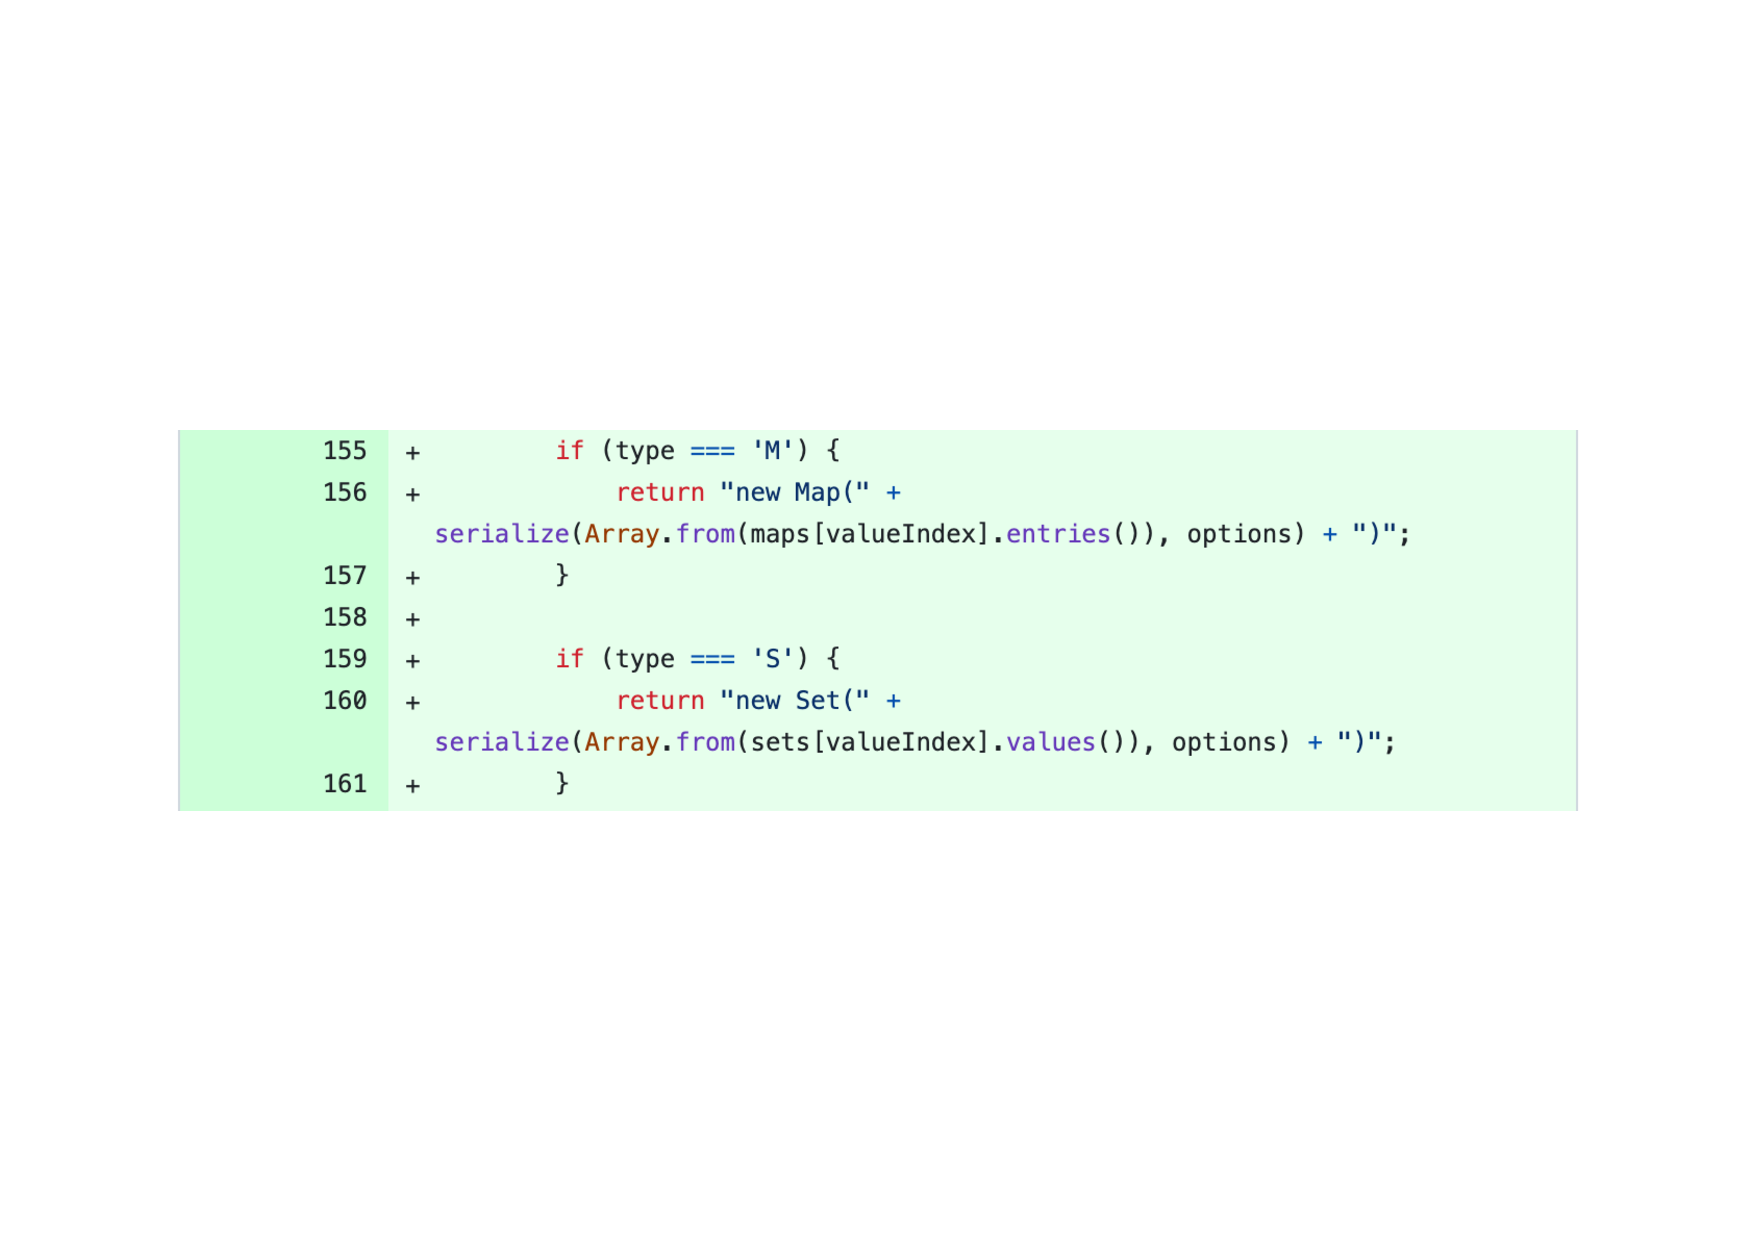
\includegraphics[width=1.0\linewidth]{fig/rq1/set-map/map.pdf}
  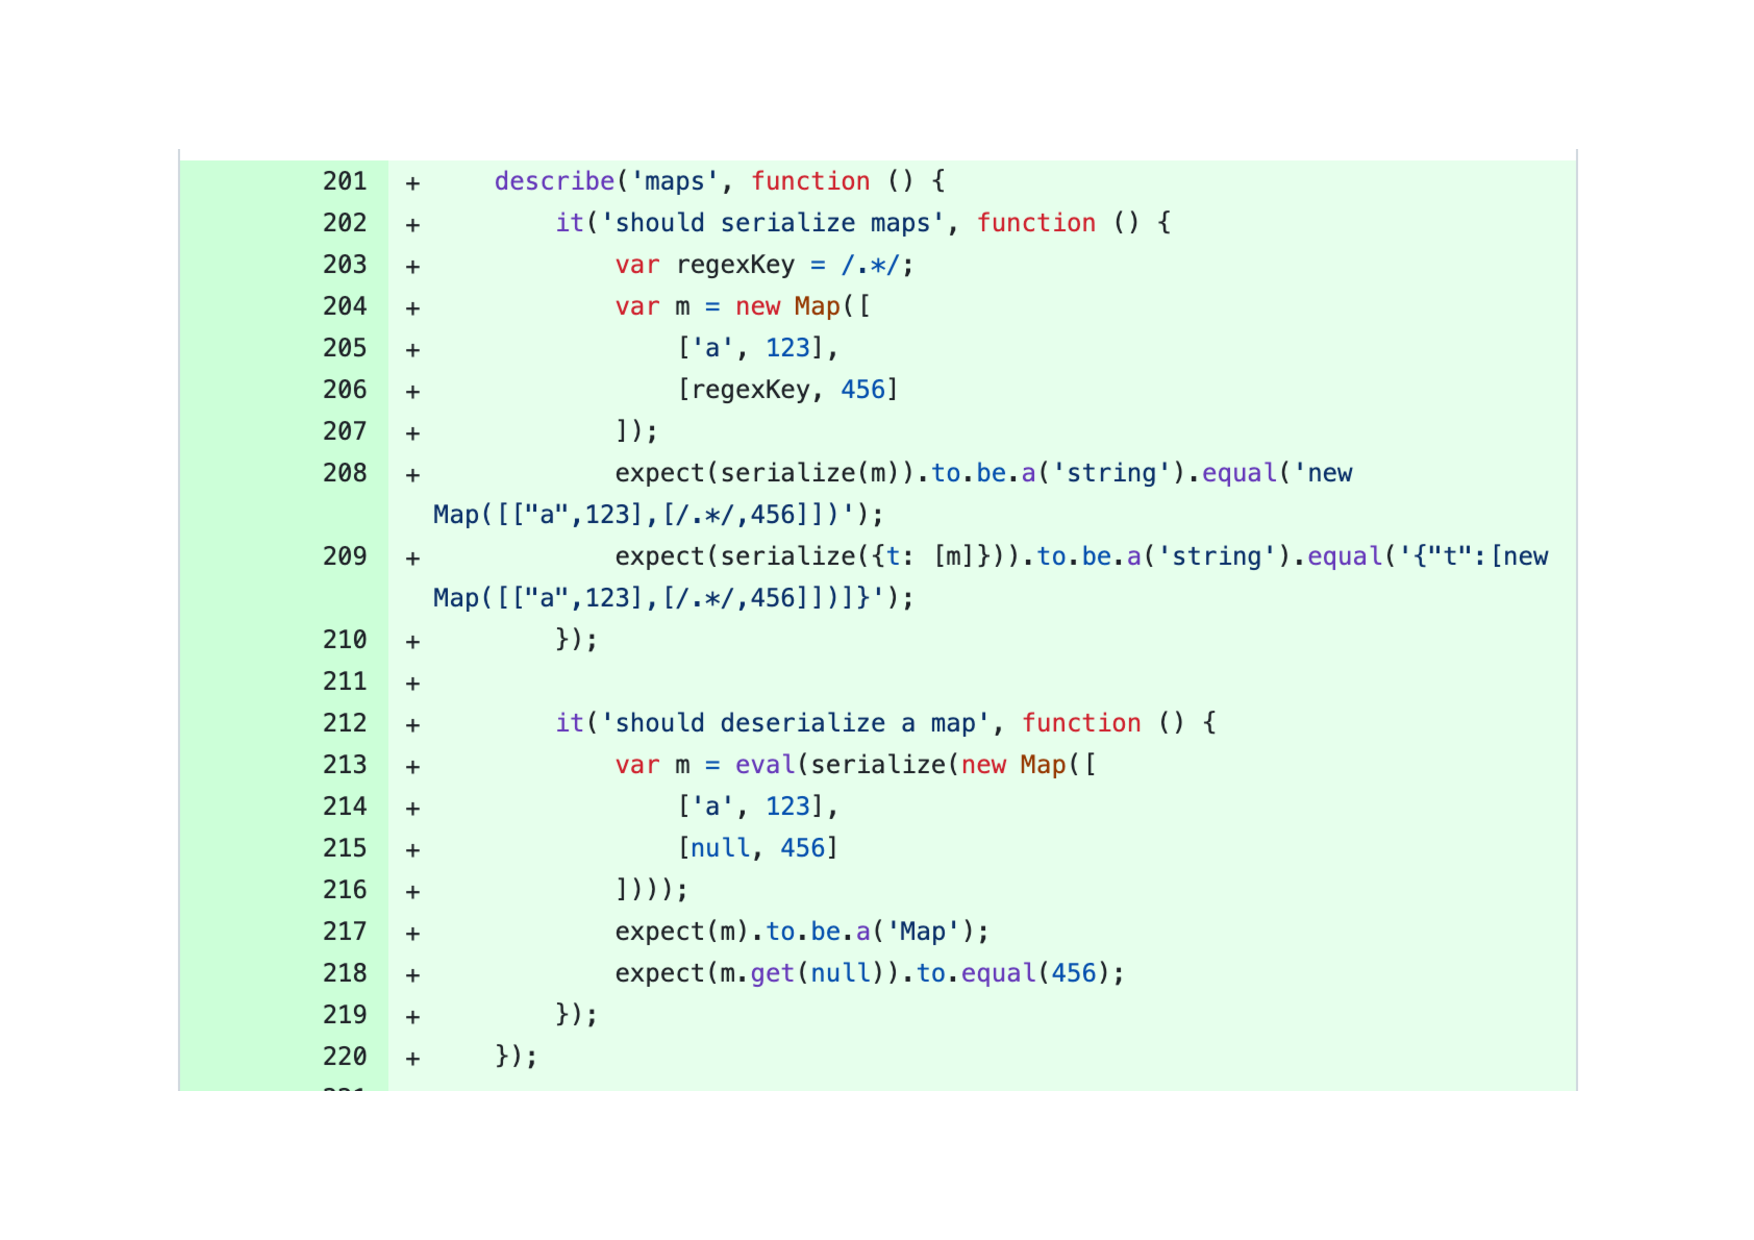
\includegraphics[width=1.0\linewidth]{fig/rq1/set-map/map.test.pdf}
  \caption{serialize-javascriptのバージョン1.6.1から1.7.0への変更}
\end{figure}

テストスイートの追加とテストケースの追加,アサーションの追加は,実際に後方互換性を保つ割合の方が高い.ただし,後方互換性の損失に伴ってテストが追加される例も存在する.後方互換性の損失に伴ってテストが追加される例として,JavaScriptオブジェクトを文字列に変換する関数を提供するライブラリserialize-javascriptのバージョン1.6.1から1.7.0への変更\footnote{\url{https://github.com/yahoo/serialize- javascript/compare/v1.6.1...v1.7.0}}を図\ref{fig:rq1.insert-test}で示す.\ref{fig:rq1.insert-test}の上部がソースコード,下部がテストコード変更内容である.

この変更では,JavaScriptでデータの集まりを扱うセット型とマップ型の入力に対し,文字列に変換する関数を適用する処理を追加している.同時に,セット型とマップ型の入力に対して文字列に正しく変換できるかを検証するテストスイートが追加されている.以前のバージョンでは,セット型とマップ型の入力に対し文字列に変換する処理がないため,文字列に変換されないことに依存しているクライアントは,バージョン更新の際に返り値が新しくなったことによる影響を受ける.このような,機能拡張による後方互換性の損失は,同時にテストが追加される場合がある.よって,機能拡張に伴うテスト追加を検出することで後方互換性の損失を捉えられると考えられる.

\subsection{テスト削除と後方互換性の損失の関係}

\begin{figure}[t]
  \label{fig:rq1.delete-test}
  \centering
  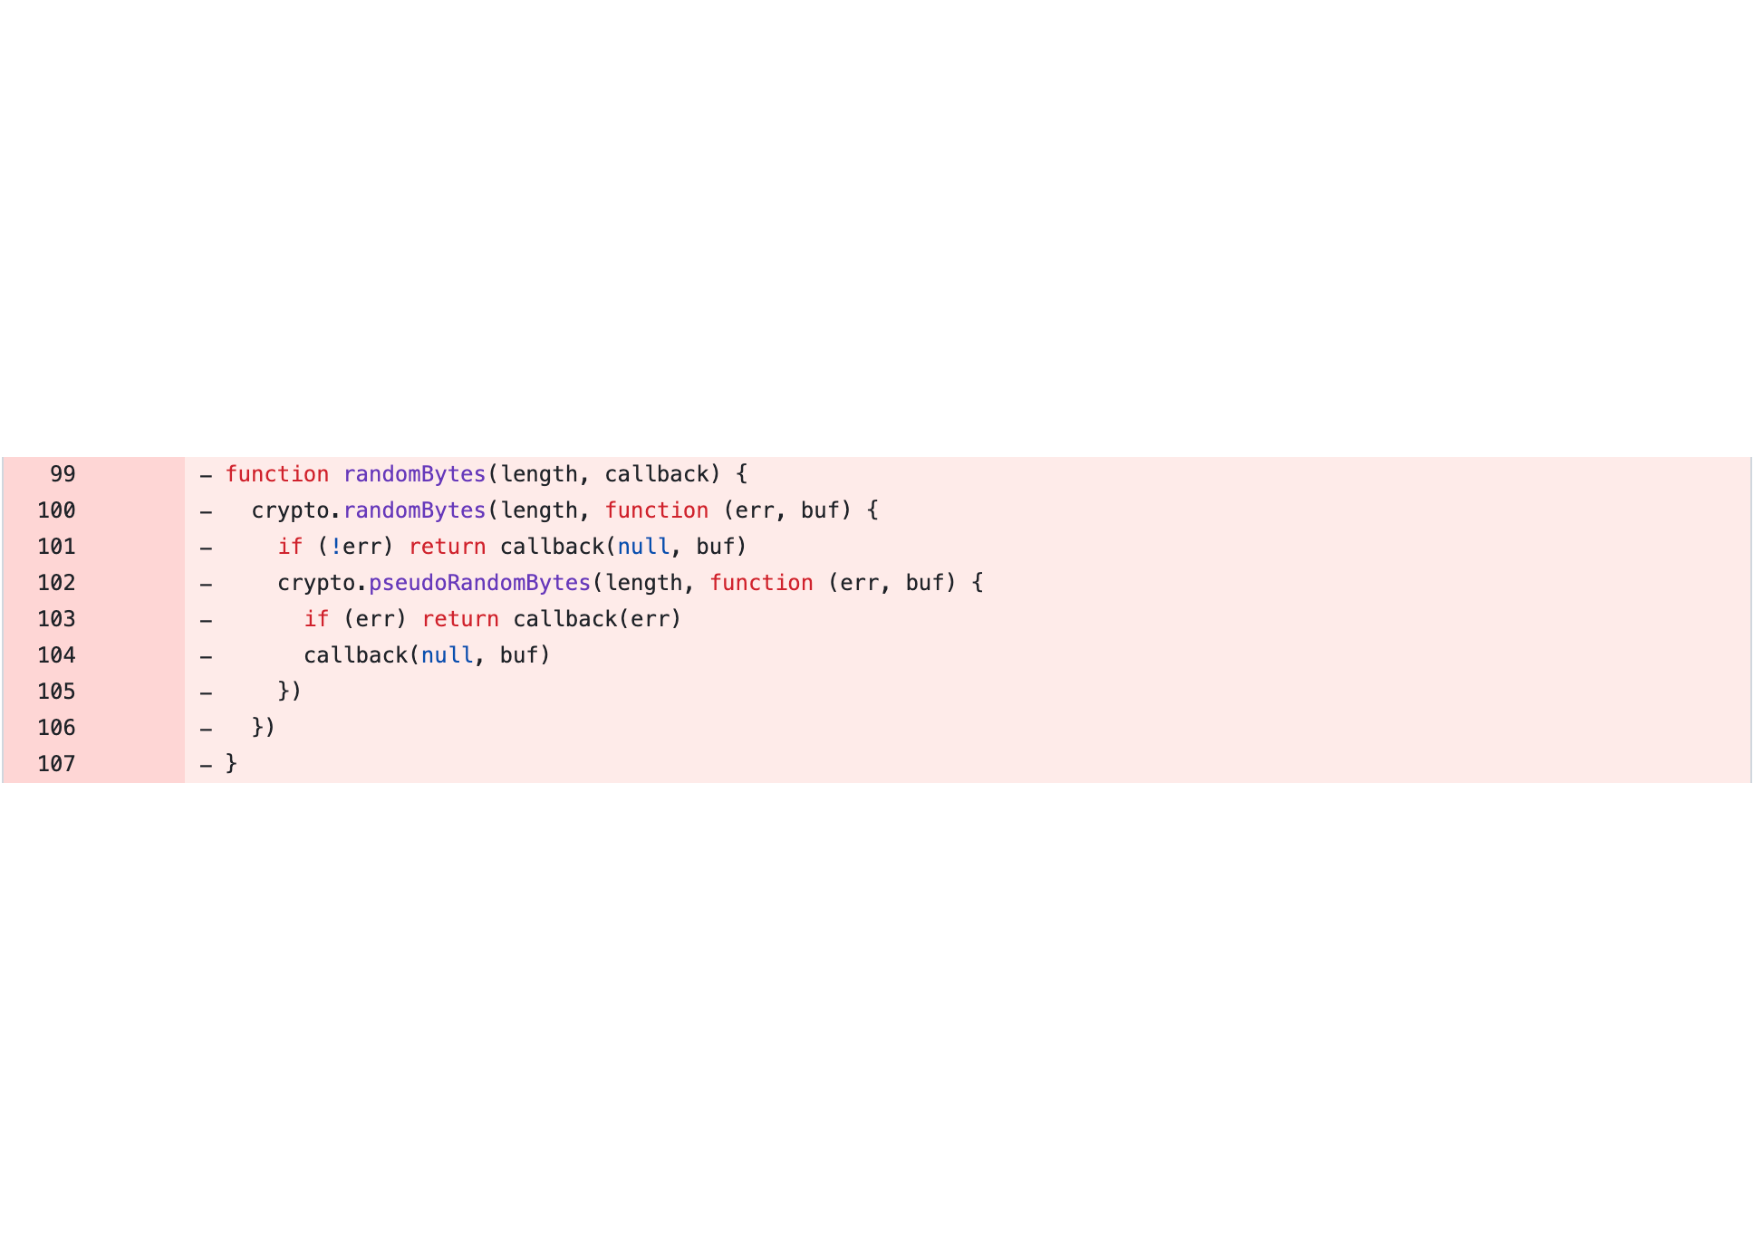
\includegraphics[width=1.0\linewidth]{fig/rq1/uuid/randomByte.pdf}
  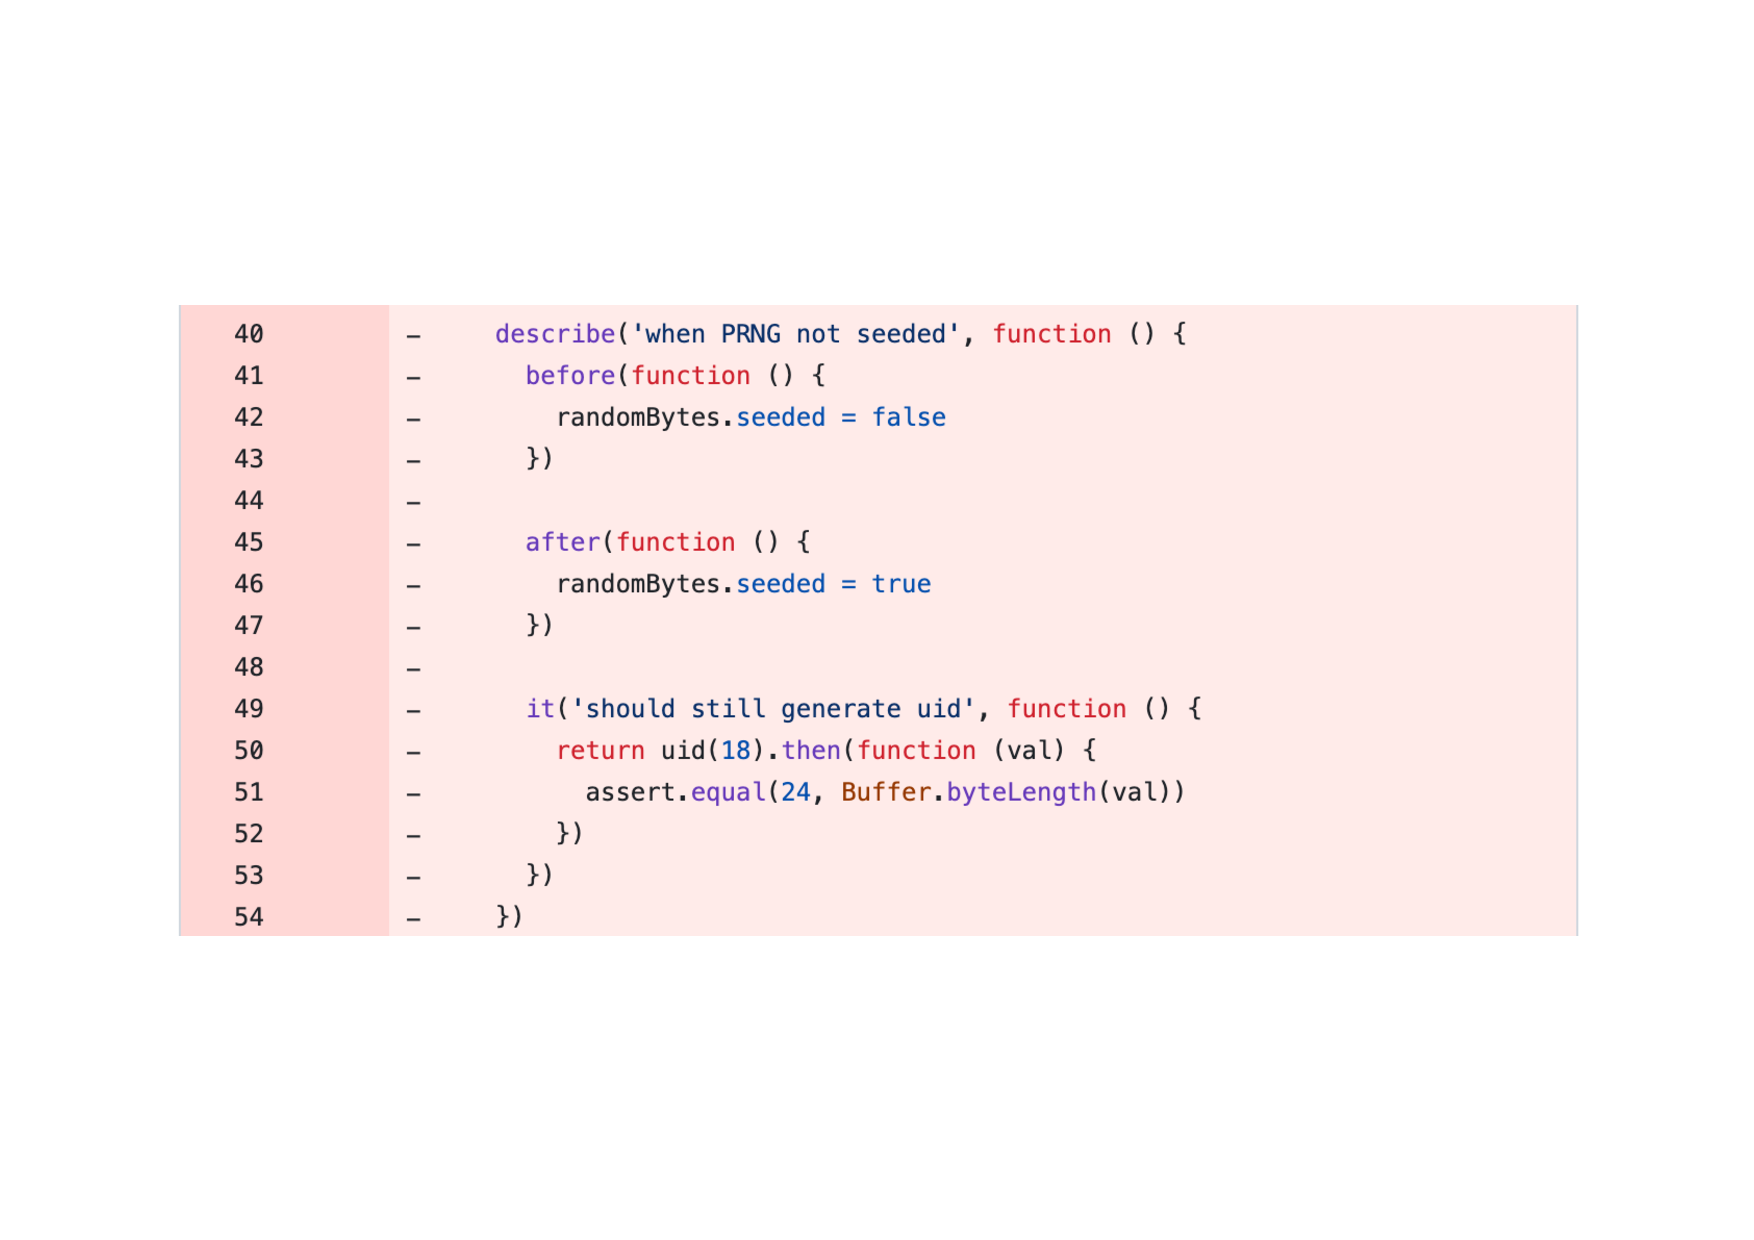
\includegraphics[width=1.0\linewidth]{fig/rq1/uuid/randomByte.test.pdf}
  \caption{uid-safeのバージョン2.0.0から2.1.0への変更}
\end{figure}

テストスイートの削除とテストケースの削除は,実際に後方互換性を損失する割合の方が高いため,テスト削除は後方互換性の損失に関係するテスト変更と言える.ただし,テストが削除されていても後方互換性の損失が検出されない場合も存在する.テストが削除されているが後方互換性の損失が検出されない例として,暗号化されたUIDを生成する関数を提供するライブラリuid-safeのバージョン2.0.0から2.1.0への変更を\footnote{\url{https://github.com/crypto-utils/uid-safe/compare/2.0.0...2.1.0}}を図\ref{fig:rq1.delete-test}で示す.図\ref{fig:rq1.delete-test}の上部がソースコード,下部がテストコード変更内容である.

この変更では,セキュリティ上の問題から,ランダムなバイト列を生成する{\verb|randomBytes|}関数を削除し,同時に{\verb|randomBytes|}の動作を検証するテストスイートを削除している.また,同バージョンで{\verb|randomBytes|}と同等のランダムなバイト列を生成するモジュールを加え,置き換えている.置き換え前後でライブラリの振る舞いが全く同じ場合,後方互換性が保たれる.また,本研究では,\ref{kouhougokanseinohantei}章で述べた通り,実際の後方互換性の判定にクライアントテストを利用している.このようなモジュールに置き換える例では,振る舞いの変化が限定的になるため,クライアントテストが捉えられず後方互換性ありと誤判定されたことが考えられる.誤判定を防ぐには実際に影響を受けるクライアントの特定が必要になるが本研究では今後の課題とする.

\subsection{アサーションの入力値,期待値の変更と後方互換性の損失の関係}

\begin{figure}[t]
  \label{fig:rq1.change-test}
  \centering
  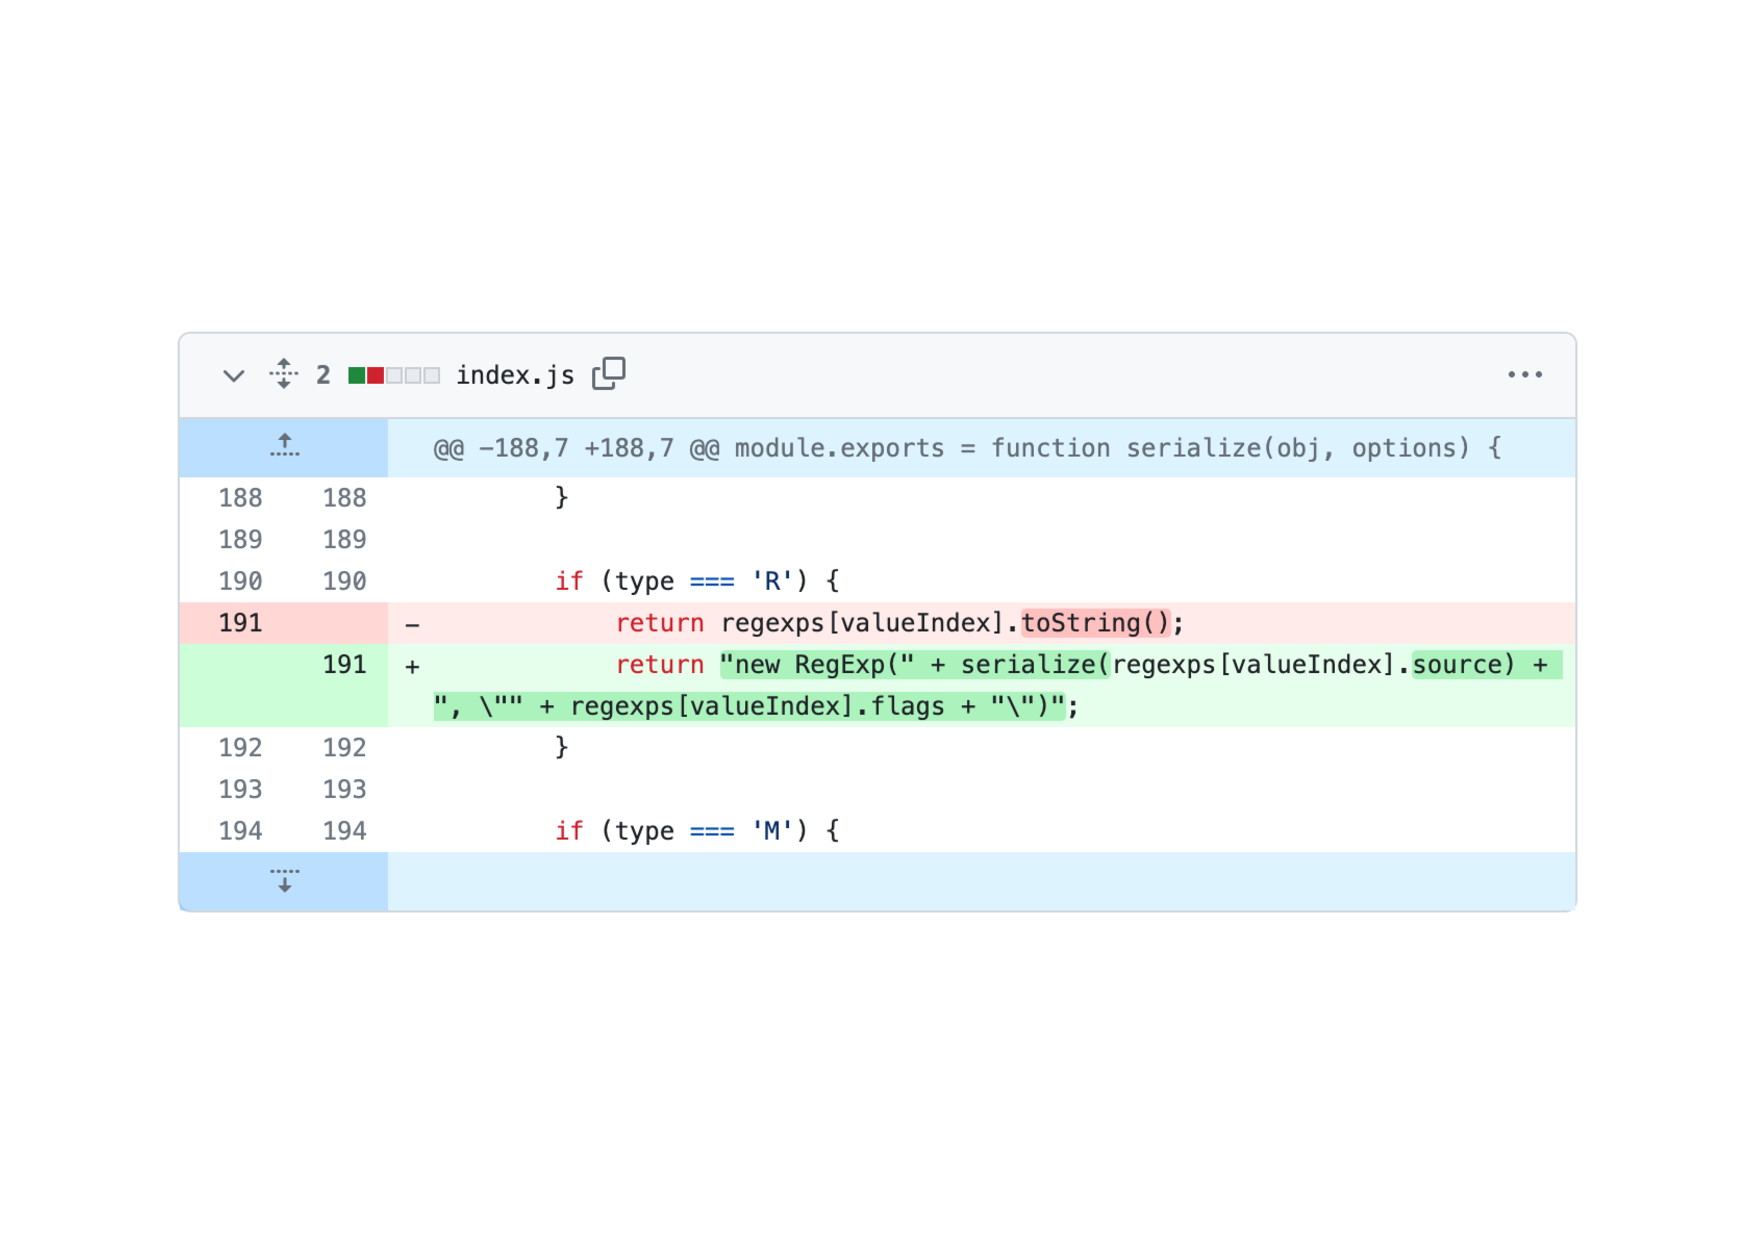
\includegraphics[width=1.0\linewidth]{fig/rq1/serialize-javascript/index.pdf}
  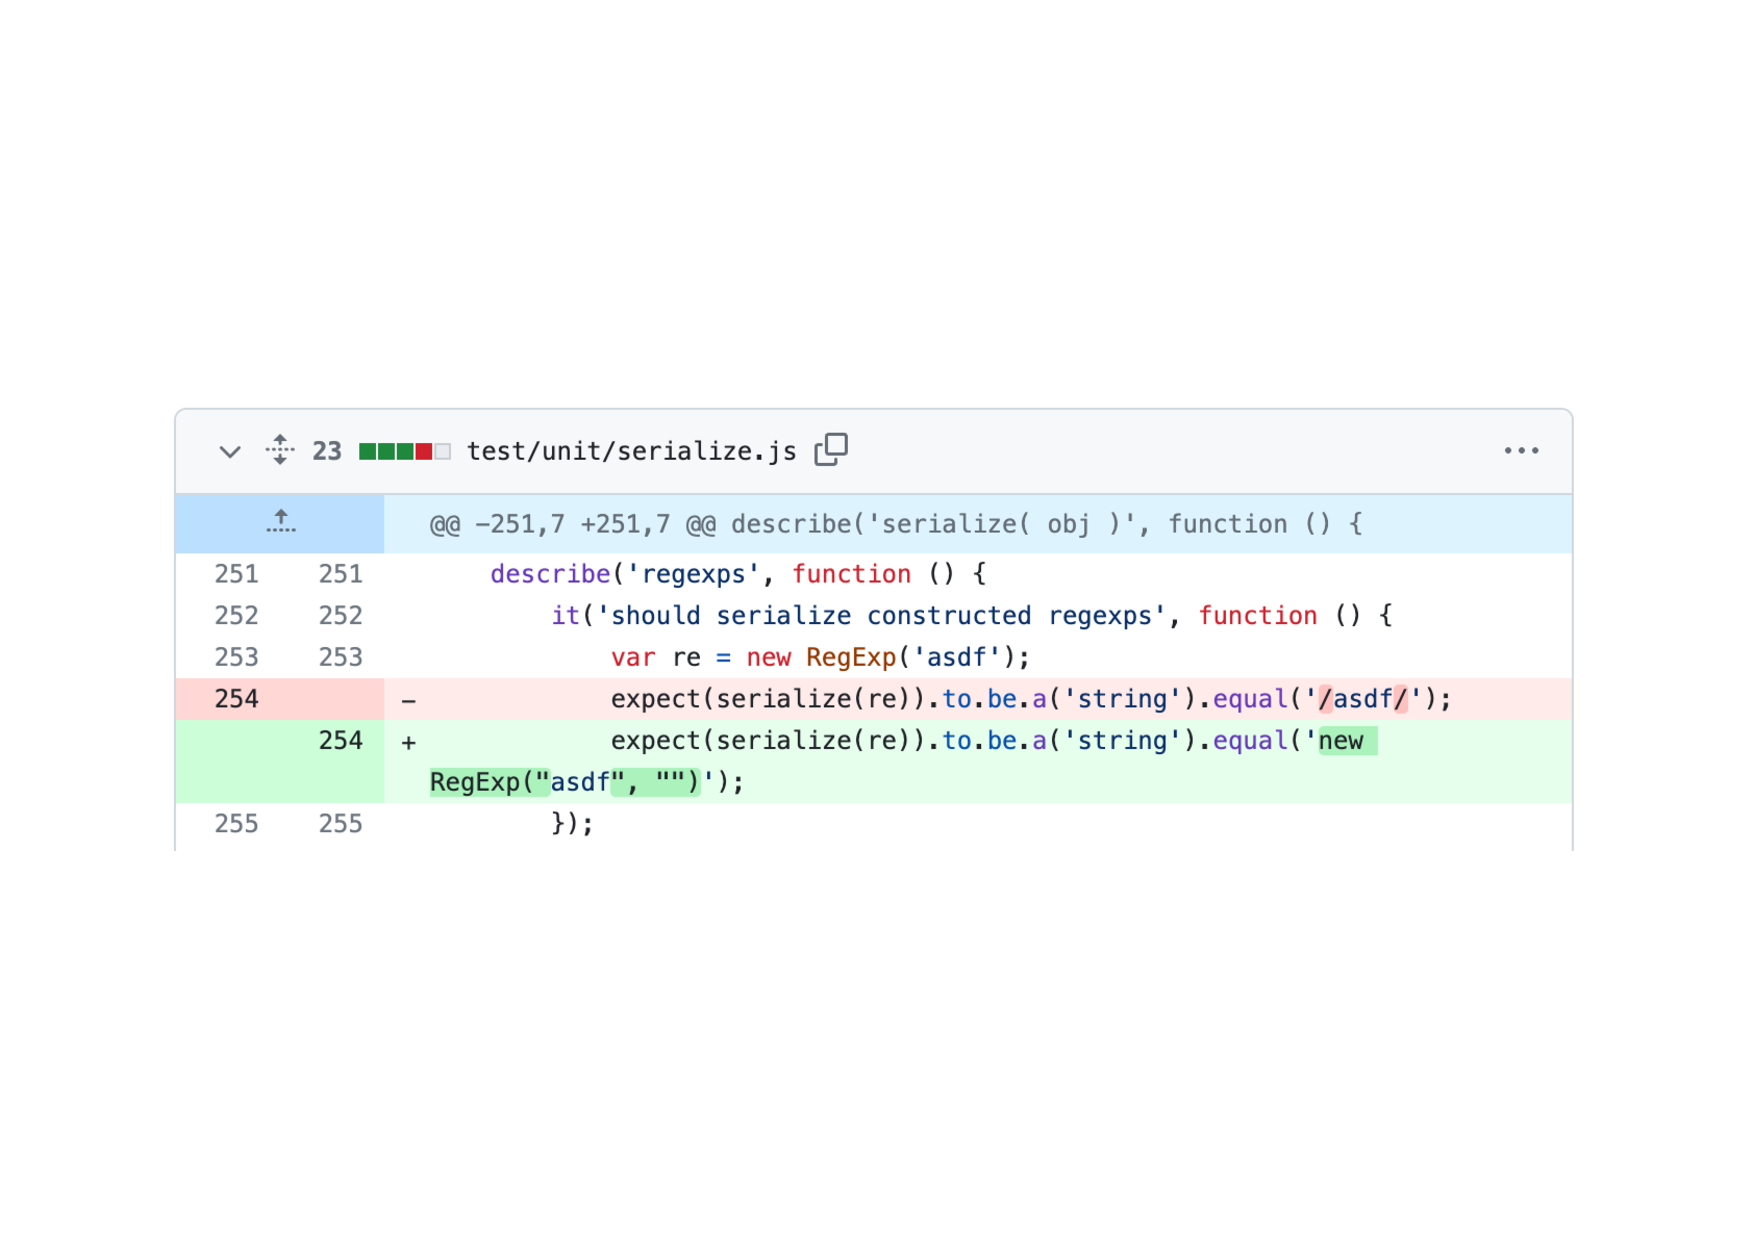
\includegraphics[width=1.0\linewidth]{fig/rq1/serialize-javascript/index.test.pdf}
  \caption{serialize-javascriptのバージョン2.1.0から2.1.1への変更}
\end{figure}

アサーションの入力値,期待値の変更は実際に後方互換性を保つ割合の方が高い.ただし,後方互換性の損失に伴ってアサーションの入力値,期待値が変更される例も存在する.後方互換性の損失に伴ってアサーションの期待値が変更される例として,serialize-javascriptのバージョン2.1.0から2.1.1への変更\footnote{\url{https://github.com/yahoo/serialize-javascript/compare/v2.1.0...v2.1.1}}を図\ref{fig:rq1.insert-test}で示す.

この変更では,セキュリティ上の問題により,正規表現に対する関数の出力が変更されている.同時に,正規表現の入力に対する返り値を検証するテストケースの期待値を変更している.よって,正規表現の入力に対して以前のバージョンでの返り値を期待するクライアントは影響を受けることがわかる.

また,後方互換性の損失に伴ってアサーションの入力値が変更される例として,CSSの色文字列を解析するライブラリcolor-stringのバージョン0.4.0から1.0.0の変更\footnote{\url{https://github.com/Qix-/color-string/compare/0.4.0...1.0.0}}では,特定の関数の使用方法が変わったことによってアサーションの入力値が変更されている.

これらの例のように,ライブラリが提供する関数の仕様変更による後方互換性の損失は,同時にアサーションの入力値や期待値が変更される場合がある.よって,仕様変更に伴うアサーションの入力値や期待値の変更を検出することで後方互換性の損失を捉えられると考えられる.

\section{まとめ}
\ref{rq1}章では,実際に後方互換性が損失した時,どのようなテスト変更が行われているかを分析した.分析により,機能拡張に伴うテスト追加,機能削除に伴うテスト削除,ライブラリが提供する関数の仕様変更に伴うアサーションの入力値,期待値の変更が後方互換性の損失に伴うテストコード変更内容であると分かった.

\chapter{RQ2:テストコード変更内容に基づく後方互換性の判定手法の有効性はどの程度か}

\section{概要}
本章では,\ref{rq1}章で述べた,後方互換性が損失するライブラリバージョンにおけるテストコード変更内容を自動検出するツールを開発し,後方互換性の損失の判定精度を従来手法と比較して検証する.まず,変更前後のソースファイルから変更されたプログラム部分と追加・削除などの変更情報を得る.その後,プログラム部分とその変更情報が特定の条件に一致すれば後方互換性が損失したと判定する.

\section{提案手法}\label{rq2:teian}

\begin{figure}[t]
  \label{fig:rq2.syuhou}
  \centering
  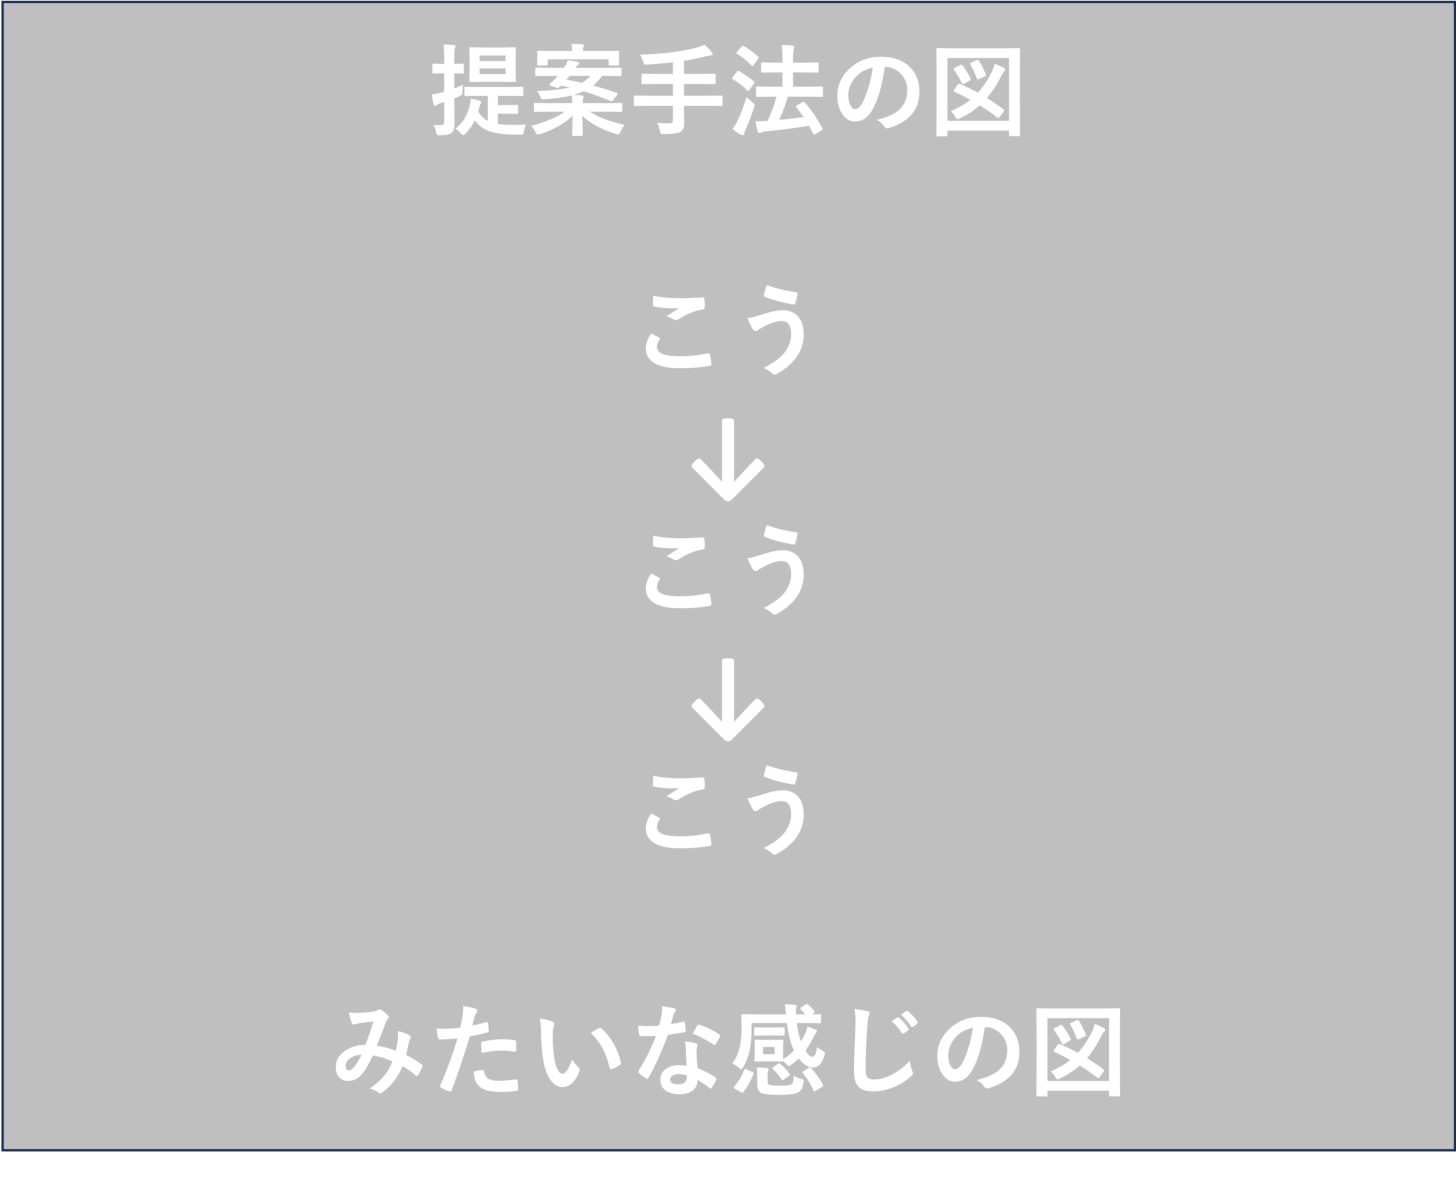
\includegraphics[width=1.0\linewidth]{fig/teiannshuhou.pdf}
  \caption{提案手法の概要}
\end{figure}

提案手法の概要を図\ref{fig:rq2.syuhou}に示す.提案手法の入力は,変更前後の全てのソースファイルであり,出力は後方互換性の有無の予測である.まず,入力として与えられた変更前後の全てのソースファイルから,変更されていないファイルを除外し,テストコードが記述されたファイルを抽出する.テストコードが記述されたファイルの条件は,ファイルパスに{\verb|test|}または{\verb|spec|}を含み,ファイル名の末尾が{\verb|.js|}または{\verb|.ts|}で,{\verb|.d.ts|}を除いたファイルとする.例えば,{\verb|test.js|}や,{\verb|spec/index.ts|}などをテストコードが記述されたファイルとして抽出する.

次に,抽出したソースファイルにおける,変更されたプログラム部分とその変更情報を\ref{astseisei}節の方法で特定する.

最後に,変更されたプログラム部分とその変更情報が\ref{rq2nojouken}節で述べる3つの条件に1つでも一致すれば,後方互換性が損失したと判定し,どれにも一致しなければ後方互換性を維持していると判定する.

\subsection{変更されたプログラム部分と変更情報の特定}\label{astseisei}
変更されたプログラム部分と変更情報の特定のために,抽象構文木(AST)ベースの差分解析ツールであるGumTree\cite{gumtree}を利用する.ASTとは,ソースコードを構文解析して得られる木構造のデータである.GumTreeは,変更前後のソースファイルまたはASTを受け取ると,それらを比較してASTのノード単位の編集操作を出力する.検出できる編集操作は,「削除」「挿入」「移動」「変更」である.GumTreeを利用する際,変更前後のファイル単位で入力すると,ファイルを横断するソースコードの移動操作に対して,「移動」ではなく,「削除と挿入」として出力されてしまうため,藤本らの手法\cite{gumtreenoyatu}を一部利用し,複数ファイルを横断した移動操作に対応させる.具体的には,以下の方法で複数ファイルを横断してGumTreeを適用する.

\begin{enumerate}
  \setlength{\itemsep}{0cm}
  \item 変更のある各ファイルごとにASTを生成する
  \item 根となるノードを1つ作成する
  \item 各ファイルごとに生成したASTを子ノードとして加えていく
  \item 1から3を変更前後で実施し,2つASTを生成する
  \item 変更前後で生成された2つのASTをGumTreeに入力して出力を得る
\end{enumerate}

以上の方法により,バージョン間のテストコード変更に対して,変更されたプログラム部分(ノード)と,「削除」「挿入」「移動」「変更」の4つの変更情報を特定することができる.

\subsection{後方互換性を損失したと予測する条件}\label{rq2nojouken}
\ref{rq1}章で述べた,「機能拡張に伴うテストコード追加」「機能削除に伴うテストコード削除」「APIの仕様変更に伴うテストコードのアサーション変更」を自動で検出するために,それぞれ条件を定義する.

まず,テストコード追加・削除を判定するために,テストコードを定義する.従来研究\cite{matsuda}では,テストファイル内に記述されている,関数名が{\verb|it|}または{\verb|test|}である関数呼び出しをテストケースとしている.本研究では,テストスイートの追加・削除を含めるため,慣習的にテストスイートの宣言として使われる{\verb|describe|}という関数名を加えた,3つの関数呼び出しをテストコードとして判定する.

次に,アサーションの変更を判定するために,アサーションを定義する.JavaScript言語では,アサーションの書き方はフレームワークによって異なる.本手法では,State of JavaScript 2022\footnote{\url{https://2022.stateofjs.com/}}で紹介されている主要なテストフレームワーク13件のうち,単体テストで使われるフレームワーク5件(Jest\footnote{\url{https://jestjs.io/}},Mocha\footnote{\url{https://mochajs.org/}},AVA\footnote{\url{https://github.com/avajs/ava}},Jasmine\footnote{\url{https://jasmine.github.io/}},Vitest\footnote{\url{https://vitest.dev/}})を考慮する.テストフレームワーク毎のアサーションの書き方は,大きく2つに大別できる.例をProgram\ref{bdd.test.js},Program\ref{tdd.test.js}で示す.

\begin{lstlisting}[caption=アサーション例1, label=bdd.test.js]
expect(calculator.add(1, 1)).to.be.a('number').equal(2);
expect(calculator.add(1, 1), 'to be', 2);
calculator.add(1, 1).should.be.a('number').equal(2);
\end{lstlisting}

Program\ref{bdd.test.js}は,自然言語に似た構文を使用してテストを記述する記述形式で,\todo{〜〜〜}で使用される.その中でも,1行目のように,{\verb|expect|}関数にメソッドチェーンで振る舞いを記述するもの,2行目のように{\verb|expect|}関数の引数にそのまま振る舞いを記述するもの,3行目のように入力に{\verb|should|}プロパティをはやして振る舞いを記述する形式がある.1,2行目の形式に対しては,{\verb|expect|}関数の第一引数を入力値,それ以降を期待値として扱い,3行目の形式に対しては,{\verb|should|}メソッド以前を入力,以降を期待値として扱う.

\begin{lstlisting}[caption=アサーション例2, label=tdd.test.js]
assert.equal(calculator.add(1, 1), 2);
t.is(calculator.add(1, 1), 2);  
t.true(calculator.add(1, 1) === 2);
\end{lstlisting}

Program\ref{tdd.test.js}は,Node.js\footnote{\url{https://nodejs.org/en}}標準の{\verb|assert|}文がメインの記述形式で,\todo{〜〜〜}で使用される.その中でも,1行目や2行目のように,第1引数に入力,第2引数に期待値を取る形式と,3行目のように入力だけを引数に取る形式がある.この形式に対しては,{\verb|assert|},{\verb|t|},{\verb|test|}をキーとして,プロパティのメソッドの第一引数を入力,第二引数を期待値として扱う.3行目のように引数が一つの場合は,引数を入力,メソッド名を期待値とする.

\subsubsection{機能拡張に伴うテストコード追加}
機能拡張に伴うテストコード追加は,GumTreeで「挿入」と判定されたノードがテストコードであり,かつ既存のテストコード中で宣言されていれば既存のAPIに新しく機能が追加されたとして,機能拡張とみなす.例えば,serialize-javascriptのバージョン1.6.1から1.7.0への変更\footnote{\url{https://github.com/yahoo/serialize- javascript/compare/v1.6.1...v1.7.0}}では,既存の{\verb|serialize( obj )|}をラベルに取るテストスイート内で,{\verb|maps|}と{\verb|sets|}をラベルに取るテストスイートが追加されているため,関数{\verb|serialize|}の機能拡張と判断し,後方互換性が損失したと判定する.

\subsubsection{機能削除に伴うテストコード削除}
機能削除に伴うテストコード削除は,GumTreeで「削除」と判定されたノードがテストコードであれば,既存のAPIが削除されたとして,機能削除とみなす.例えば,uid-safeのバージョン2.0.0から2.1.0への変更\footnote{\url{https://github.com/crypto-utils/uid-safe/compare/2.0.0...2.1.0}}では,既存の{\verb|when PRNG not seeded|}をラベルに取るテストスイートが削除されているため,このテストスイート内でテストされている項目に対応する機能が削除されたとして,後方互換性が損失したと判定する.

\subsubsection{APIの仕様変更に伴うテストコードのアサーション変更}
APIの仕様変更に伴うテストコードのアサーション変更は,GumTreeで「変更」と判定されたノードが,アサーションの入力値または期待値であれば,APIの仕様が変更されたとみなす.この時,入力値と期待値が同時に変更されている場合は,同じテストケースをカバーするアサーションのリファクタリングと考えられるため,無視する.例えば,\todo{〜〜〜}の変更では,\todo{〜〜〜ため}後方互換性を損失したと判定する.一方,\todo{〜〜〜}の変更は,\todo{〜〜〜ため},後方互換性を損失したと判定しない.

\section{データセット}
データセットとして,\ref{rq1:datasets}章と同様,従来研究\cite{matsuda}で収集されたライブラリバージョン2,111件のうち,削除や非公開になったことによりGitHub上でアクセスできないものと,GumTree上でエラーになるもの計156件を除いた1,955件を使用する.

\section{分析結果}

データセットに対して,従来手法と,\ref{rq2:teian}章で述べた手法を適用した.結果を表\ref{fig:result}に示す.分析対象とするライブラリバージョン1,955件中,提案手法で後方互換性なしと予測したライブラリバージョンは662件(約34%),後方互換性ありと予測したライブラリバージョンは1,293件(約66%)であった.また,従来手法で後方互換性なしと予測したライブラリバージョンは905件(約46%),後方互換性ありと予測したライブラリバージョンは1,050件(54%)であった.

提案手法で後方互換性を損失したと予測したライブラリバージョン662件中,114件(約17%)は後方互換性を損失し,662件中548件(約83%)は後方互換性を維持している.また,後方互換性を損失したライブラリバージョン223件中,114件(約51%)を正しく予測した.従来手法では,後方互換性を損失したと予測したライブラリバージョン905件中,140件(約15%)が後方互換性を損失し,後方互換性を損失したライブラリバージョン223件中.140件(63%)を正しく予測した.

従来手法で後方互換性なしと判定したライブラリバージョン中765件が誤判定だったのに対し,提案手法では548件が誤検出であった.これは,従来手法で誤検出となる,テストケースの移動やラベルの修正などのテストコードのリファクタリングによる影響を提案手法では受けないため,誤検出を減らすことができたことを示している.一方で,提案手法は従来手法に比べて,後方互換性を損失したライブラリバージョンの検出精度が低下している.従来手法では後方互換性を損失したライブラリバージョン223件中、140件を正確に検出できたのに対し、提案手法では114件のみを検出した。この結果から、提案手法は誤検出を減らすことには成功しているが、後方互換性を損失したライブラリバージョンの検出においては改善の余地があるとわかる。

予測結果を目視により調査した内容については,\ref{rq2:kousatu}章で言及する.

\begin{table}[]
  \centering
  \label{fig:result}
  \begin{tabular}{l|r|r|r}
    \hline
                    & \multicolumn{1}{c|}{後方互換性なし} & \multicolumn{1}{c|}{後方互換性あり} & \multicolumn{1}{c}{合計} \\ \hline
    後方互換性なしと予測      & 114                          & 548                          & 662                    \\ \hline
    後方互換性ありと予測      & 109                          & 1,184                        & 1,293                  \\ \hline
    合計              & 223                          & 1,732                        & 1,955                  \\ \hline\hline
    従来手法で後方互換性なしと予測 & 140                          & 765                          & 905                    \\ \hline
    従来手法で後方互換性ありと予測 & 83                           & 967                          & 1,050                  \\ \hline
    合計              & 223                          & 1,732                        & 1,955                  \\ \hline
  \end{tabular}
\end{table}


\section{考察}\label{rq2:kousatu}
分析したライブラリバージョンを目視で確認し,ライブラリバージョンの例を挙げて分析結果の適合率と再現率について考察する.













\section{まとめ}






\chapter{妥当性への脅威}

\section{内的妥当性}

\section{外的妥当性}

\chapter{おわりに}

\chapter*{謝辞}

% 文献を参照する場合には,論文の最後に参考文献として列挙するとともに,
% \verb|\cite|を使って,例えば,
% \begin{quote}
%   文献\cite{1390850475731067264}によれば…
% \end{quote}
% や,
% \begin{quote}
%   …である\cite{latex2e}.
% \end{quote}
% のように参照する.

% 文献の列挙には,{\tt thebibliography}環境などを用いる\footnote{使い方
%   は,この資料のソースを参照.}.

%%%%%%%%%%%%%%%%%%%%%%%%%%%%%%%%%%%%%%%%%%%%%%%%%%%%%%%%%%%%%%%%%%%%%%%%

%%
%% 謝辞
%%
%% \begin{acknowledgements}
%% 感謝します.
%% \end{acknowledgements}

%%%%%%%%%%%%%%%%%%%%%%%%%%%%%%%%%%%%%%%%%%%%%%%%%%%%%%%%%%%%%%%%%%%%%%%%

%%
%% 参考文献
%%

\bibliographystyle{junsrt}
\bibliography{thesis}

%%%%%%%%%%%%%%%%%%%%%%%%%%%%%%%%%%%%%%%%%%%%%%%%%%%%%%%%%%%%%%%%%%%%%%%%

%%
%% 付録
%%
% \appendix
% 
% \chapter{サンプルプログラム}
% 
% プログラムリストや実行結果など,本論を補足する上で必要と思われるものが
% あれば付録として付ける.
% 
% {
% \footnotesize
% \begin{verbatim}
% #include <stdio.h>
% int main(void)
% {
%     printf("Hello, World!\n");
%     return 0;
% }
% \end{verbatim}
% }

%%%%%%%%%%%%%%%%%%%%%%%%%%%%%%%%%%%%%%%%%%%%%%%%%%%%%%%%%%%%%%%%%%%%%%%%

\end{document}
